\subsection{Backend: Bildverarbeitung}
Im Folgenden Abschnitt werden die wichtigsten Klassen und Funktionen des Backends vorgestellt. Diese sind auch in Abbildung \ref{fig:backend} dargestellt.
\FloatBarrier
\begin{figure*}
    \centering
    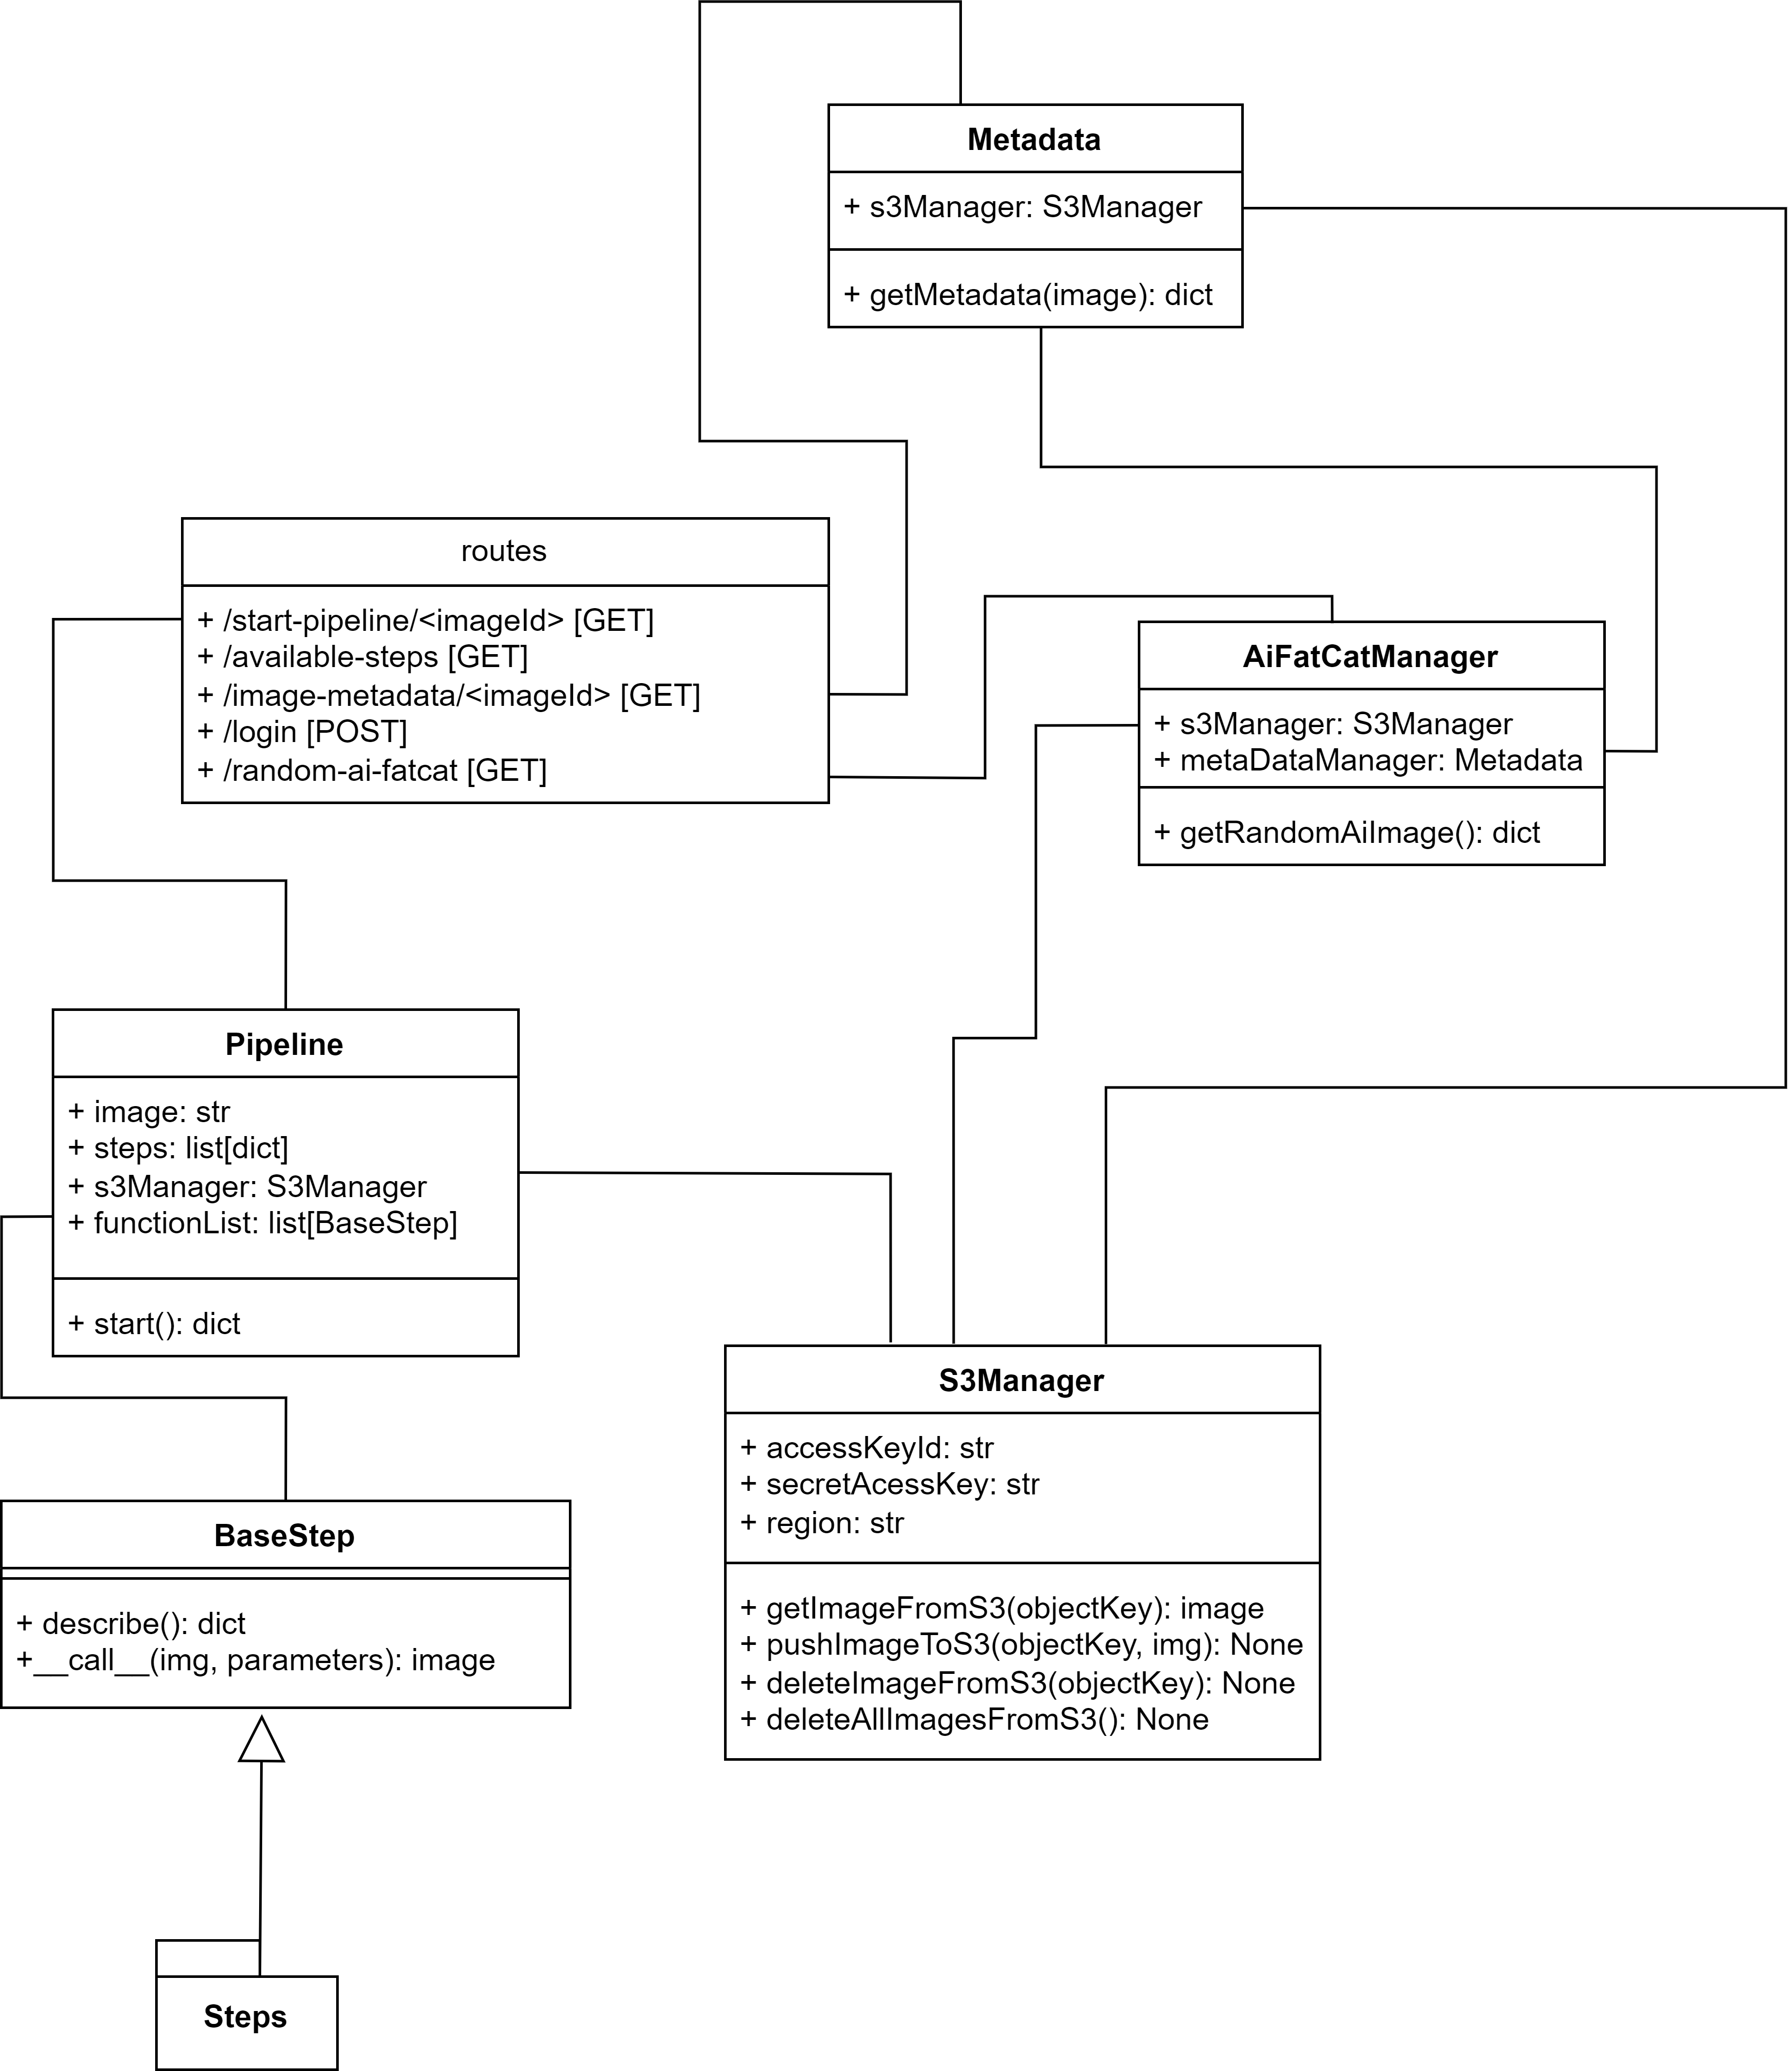
\includegraphics[width=.7\textwidth]{Bilder/BackendBDCC.png}
    \caption{Die wichtigsten Klassen und Funktionen im Backend}
    \label{fig:backend}
\end{figure*}
\textbf{routes:} Hier werden alle REST-Endpunkte definiert um die Schnittstelle zum Frontend zu ermöglichen. Der Endpunkt \glqq /start-pipeline/\textless imageId\textgreater \grqq{} ist dabei dafür zuständig die Verarbeitung eines Bildes zu starten. \glqq \textless imageId\textgreater  \grqq{} ist dabei eine eindeutie ID um das zu verarbeitende Bild aus dem S3-Bucket zu laden. Im Content des HTTP-POST Requests werden dabei die auszuführenden Pipeline-Schritte, sowie deren Parameter übergeben. Die tatsächliche Verarbeitung des Bilds übernimmt die Klasse \glqq Pipeline\grqq{}.
Der Endpunkt \glqq /available-steps\grqq{} liefert eine Beschreibung für alle Implementierten Pipeline-Steps, sowie deren Parameter. Dieser Endpunkt wird verwendet um die verfügbaren Verarbeitungsschritte im Frontend anzuzeigen und dem Benutzer Informationen über deren Verwendung zu liefern.
Mit Hilfe des Endpunkts \glqq /image-metadata/\textless imageId\textgreater \grqq{} kann ein Histogramm für das übergebene Bild erstellt werden. Außerdem liefert der Endpunkt Informationen über die Größe des Bilds und die Anzahl an Farbkanälen. Für die Erzeugung dieser Informationen ist die Klasse \glqq Metadata\grqq{} verantwortlich.
Der Endpunkt \glqq /login\grqq{} liefert stellt die Möglichkeit die im POST-Request übergebenen Parameter Benutzername und Passwort zu überprüfen. Dieser wird verwendet um dem Benutzer die Möglichkeit zu geben das Entwicklermenü im Frontend zu aktivieren und darüber alle Daten aus dem S3-Bucket zu löschen. In der Aktuellen Implementierung werden Benutzername und Passwort im Klartext unverschlüsselt über HTTP übertragen. Diese Übertragung stellt keine sichere Authentifizierung dar für den Einsatz in einem Produktivsystem muss an dieser Stelle eine sichere Authentifizierung implementiert werden.
Unter dem Endpunkt \glqq /random-ai-fatcat\grqq{} kann ein zufälliges Katzenbild aus dem Internet geladen werden. Dieses wird im S3-Bucket gespeichert und die ID zurückgegeben. Die Bilder stammen dabei von \glqq https://thecatapi.com\grqq{}. 

\textbf{S3Manager:} Die Klasse \glqq S3Manager\grqq{} stellt Methoden zur Verfügung um mit einem S3-Bucket zu interagieren bereit.Die Methode \glqq getImageFromS3\grqq kann verwendet werden um ein Bild aus dem S3-Bucket zu laden. Die Methode bekommt dafür den \glqq objectKey\grqq{}, also eine eindeutiege ID, übergeben. Mit Hilfe der Methode \glqq pushImageToS3\grqq{} kann ein Bild unter einem bestimmten \glqq objectKey\grqq{} im S3-Bucket abgelegt werden. Außerdem werden die Methoden \glqq deleteImageFromS3\grqq{} und \glqq deleteAllImagesFromS3\grqq{} bereitgestellt, um ein bestimmtes oder alle Bilder aus dem S3-Bucket zu löschen. 

\textbf{Metadata:} Die Klasse \glqq Metadata\grqq{} ist für die Erzeugung des Histogramms, sowie für die Extraktion von Metadaten aus einem Bild verantwortlich. Zu diesem Zweck stellt die Klasse die Methode \glqq getMetadata\glqq zur Verfügung. Diese bekommt als Eingabe ein Bild. Die Methode erzeugt ein Histogramm und speichert dieses als Bild im S3-Bucket. Zurückgegeben wird eine ID unter der das erzeugte Histogramm abgerufen werden kann, die Breite und Höhe des Bildes, sowie die Anzahl an Farbkanälen. 

\textbf{Pipeline:} Die zentrale Klasse zum verarbeiten der Bilder ist die Klasse \glqq Pipeline\grqq{}. Diese wird für jede Verarbeitung neu initialisiert. Bei der Initialisierung bekommt sie bereits die ID des zu verarbeitenden Bilds, sowie die Verarbeitungsschritte die Ausgeführt werden sollen mit. Beim Aufruf der Methode \glqq start\grqq{} wird über die Liste aller übergebenen Schritte iteriert und dieses mit den entsprechenden Parametern ausgeführt. Dabei sind alle Schritte von der Klasse \glqq BaseStep\grqq{} abgeleitet. Als Eingabe für den nächsten Verarbeitungsschritt dient dabei die Ausgabe des Vorherigen. Jedes Zwischenergebniss wird im S3-Bucket abgespeichert. Außerdem werden Histogramm und Metadaten für jedes Zwischenergebniss generiert. Die Methode liefert eine liste an IDs und Metadaten für alle Zwischenergebnisse, diese können im Frontend angezeigt werden.

\textbf{BaseStep:} Die Klasse \glqq BaseStep\grqq{} stellt das Grundgerüst für alle implementierten Schritte dar. Alle Schritte implementieren die Methode \glqq \_\_call\_\_\grqq{}, die die Verarbeitung eines Bildes mit den übergebenen Parametern ausführt und das Ergebnissbild zurückliefert. Außerdem implementieren alle Schritte die Methode \glqq describe\grqq{}  diese liefert Informationen über die Benutzung des Schritts und wird verwendet um dem Benutzer die Schritte im Frontend zu erklären und anzuzeigen (siehe: Endpunkt \glqq/available-steps\grqq{})